\section{Background estimation}
\label{Sec:BkgEst}

As outlined above, the largest background in the search regions originates from the \ttbar production, where both top quarks decay leptonically ($\ttbar\rightarrow 2l$) and one of the leptons is not identified due to limited detector acceptance or inefficiency of the identification requirements. A smaller contribution to the lost lepton background comes from single t production in association with a W boson.  The lost lepton background is estimated using a dileptonic control region.  The SM background with one real lepton comes from W decays, either through direct W production or via W bosons from top decays.  The neutrino from the W decay is the dominant source of real \MET.  Our baseline cuts of $\MET>250 \GeV$ and $\MT>150 \GeV$ suppress this background significantly.    The suppression is smaller for the direct W bosons because the top mass functions as a kinematic constraint on the W mass in \ttbar. As a result, the high transverse mass tail in ttbar 1-lepton events is dominated by \MET resolution effects, while for W+jets it is largely driven by physics, i.e. the width of the W.   In the search regions where the contribution from W+jets background is significant, we predict the background by extrapolating from a control region with a b-jet veto.  In the other search regions and for the ($\ttbar\rightarrow 1l$) background we rely on the simulation.  Finally also some SM processes with small cross sections will be part of the background to the search.  The dominant one is \ttbar production in association with a Z boson, where the Z boson decays into two neutrinos.  Smaller contributions come from the other processes where \ttbar is produced in association with a vector boson ($\ttbar$W, \ttbar$\gamma$), and processes with two or three electroweak vector bosons. Multijet backgrounds are negligible in this search because we require a high-$\pt$ lepton, large \MET, large \MT, at least 1 b-tagged jet and a large azimuthal angle between the \MET and the two highest-$\pt$ jets.

\subsection{Lost lepton background}\label{sec:dilepton}
The lost lepton background is estimated from data in a control region that requires a second lepton, passing the veto requirements, or the presence of an isolated track or tau.  After the simulation is corrected for differences in the lepton and jet reconstruction efficiencies, we can estimate the contribution in the search region by extrapolating from this data control region using a transfer factor taken from the simulation.   To prevent signal contamination in the tails of \MET and to increase the number of events available for the measurement in the control regions, we decided to only bin in low and high \MTtW and use an additional transfer factor for the binning in jet multiplicity and \MET. This second transfer factor is checked in dedicated studies by validating the modeling of additional jets due to initial- and final-state-radiation and the modeling of the \MET spectrum.   Figure \ref{fig:dilepton} shows good agreement between data and simulation in the dilepton control region for the \MET and \MTtW distributions.

\begin{figure}[ht]
\centering
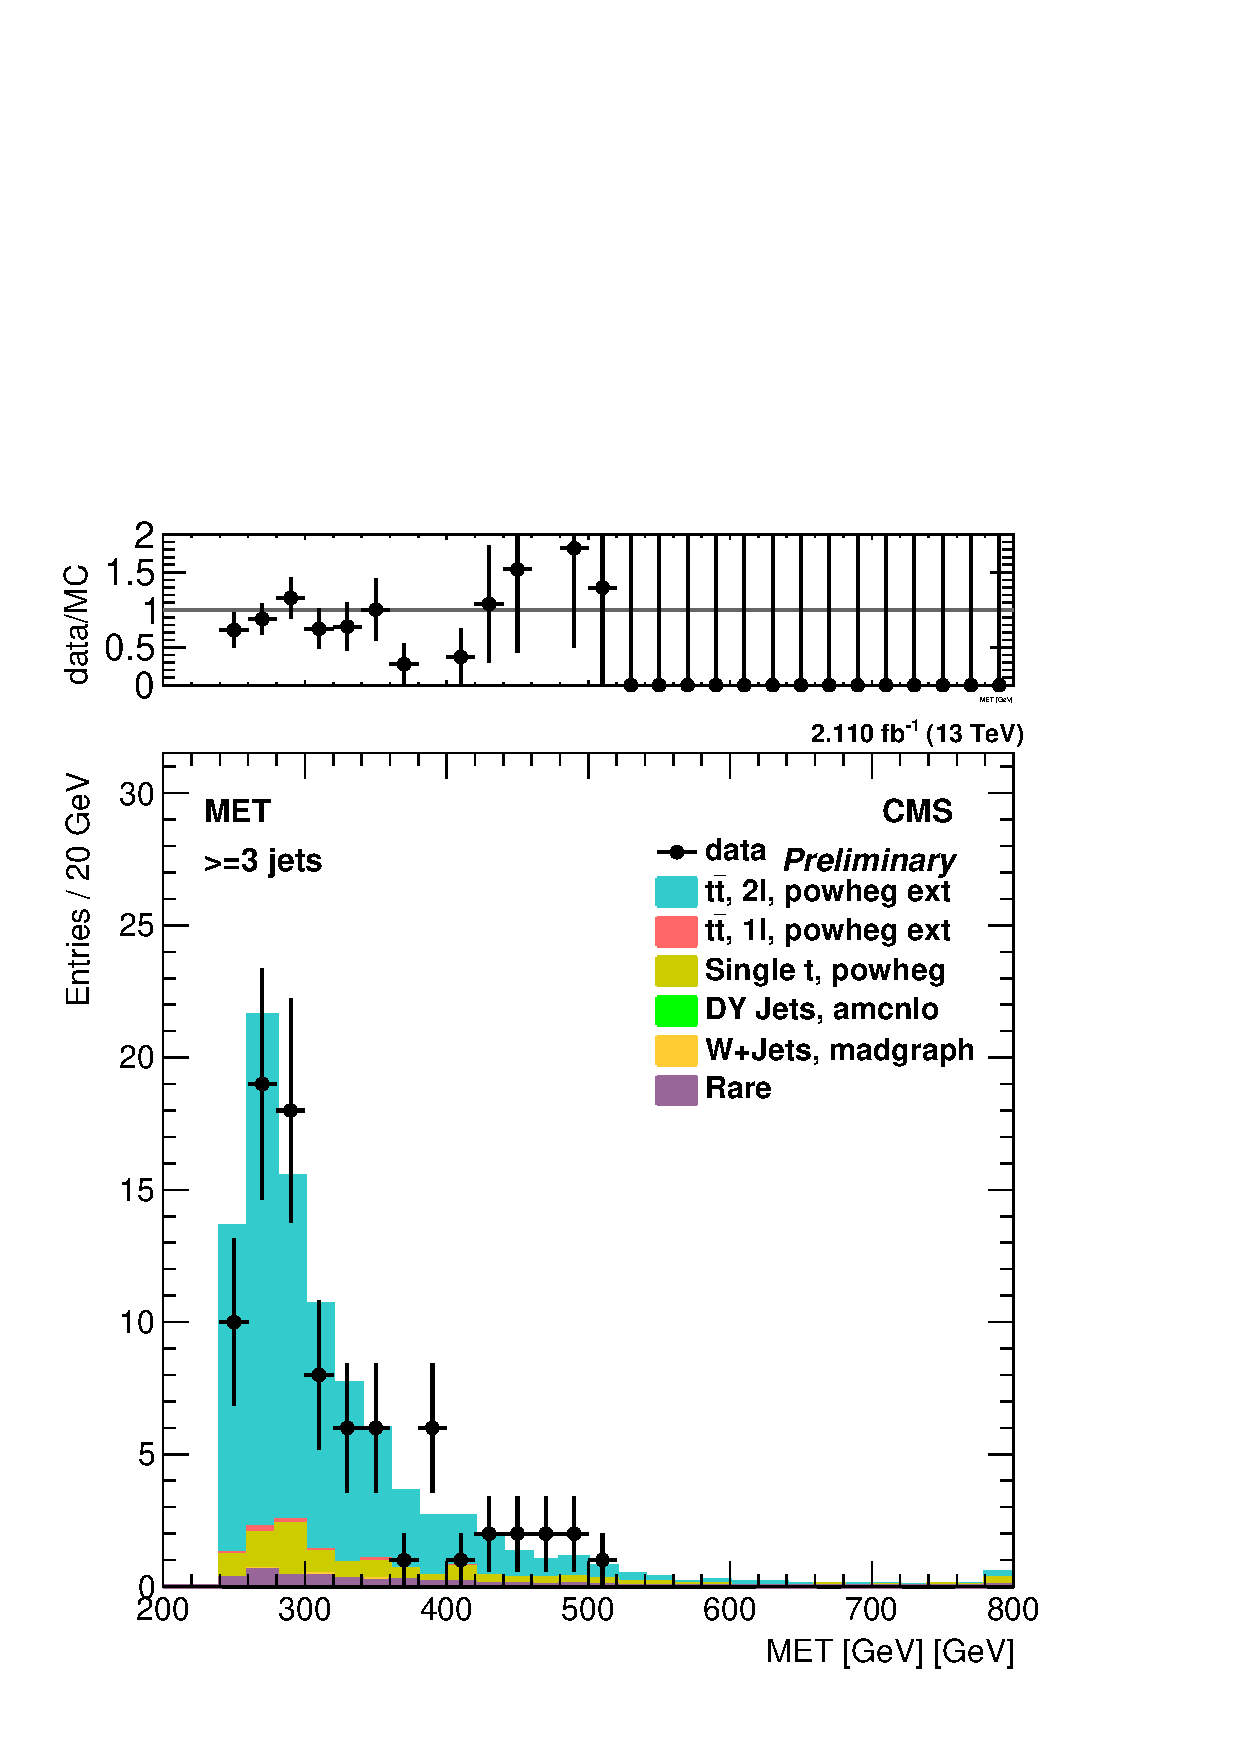
\includegraphics[width=0.45\textwidth]{plots_stop/data_MC_plot__byProductionMode__met__ge3j_ge250met__linScale.pdf}
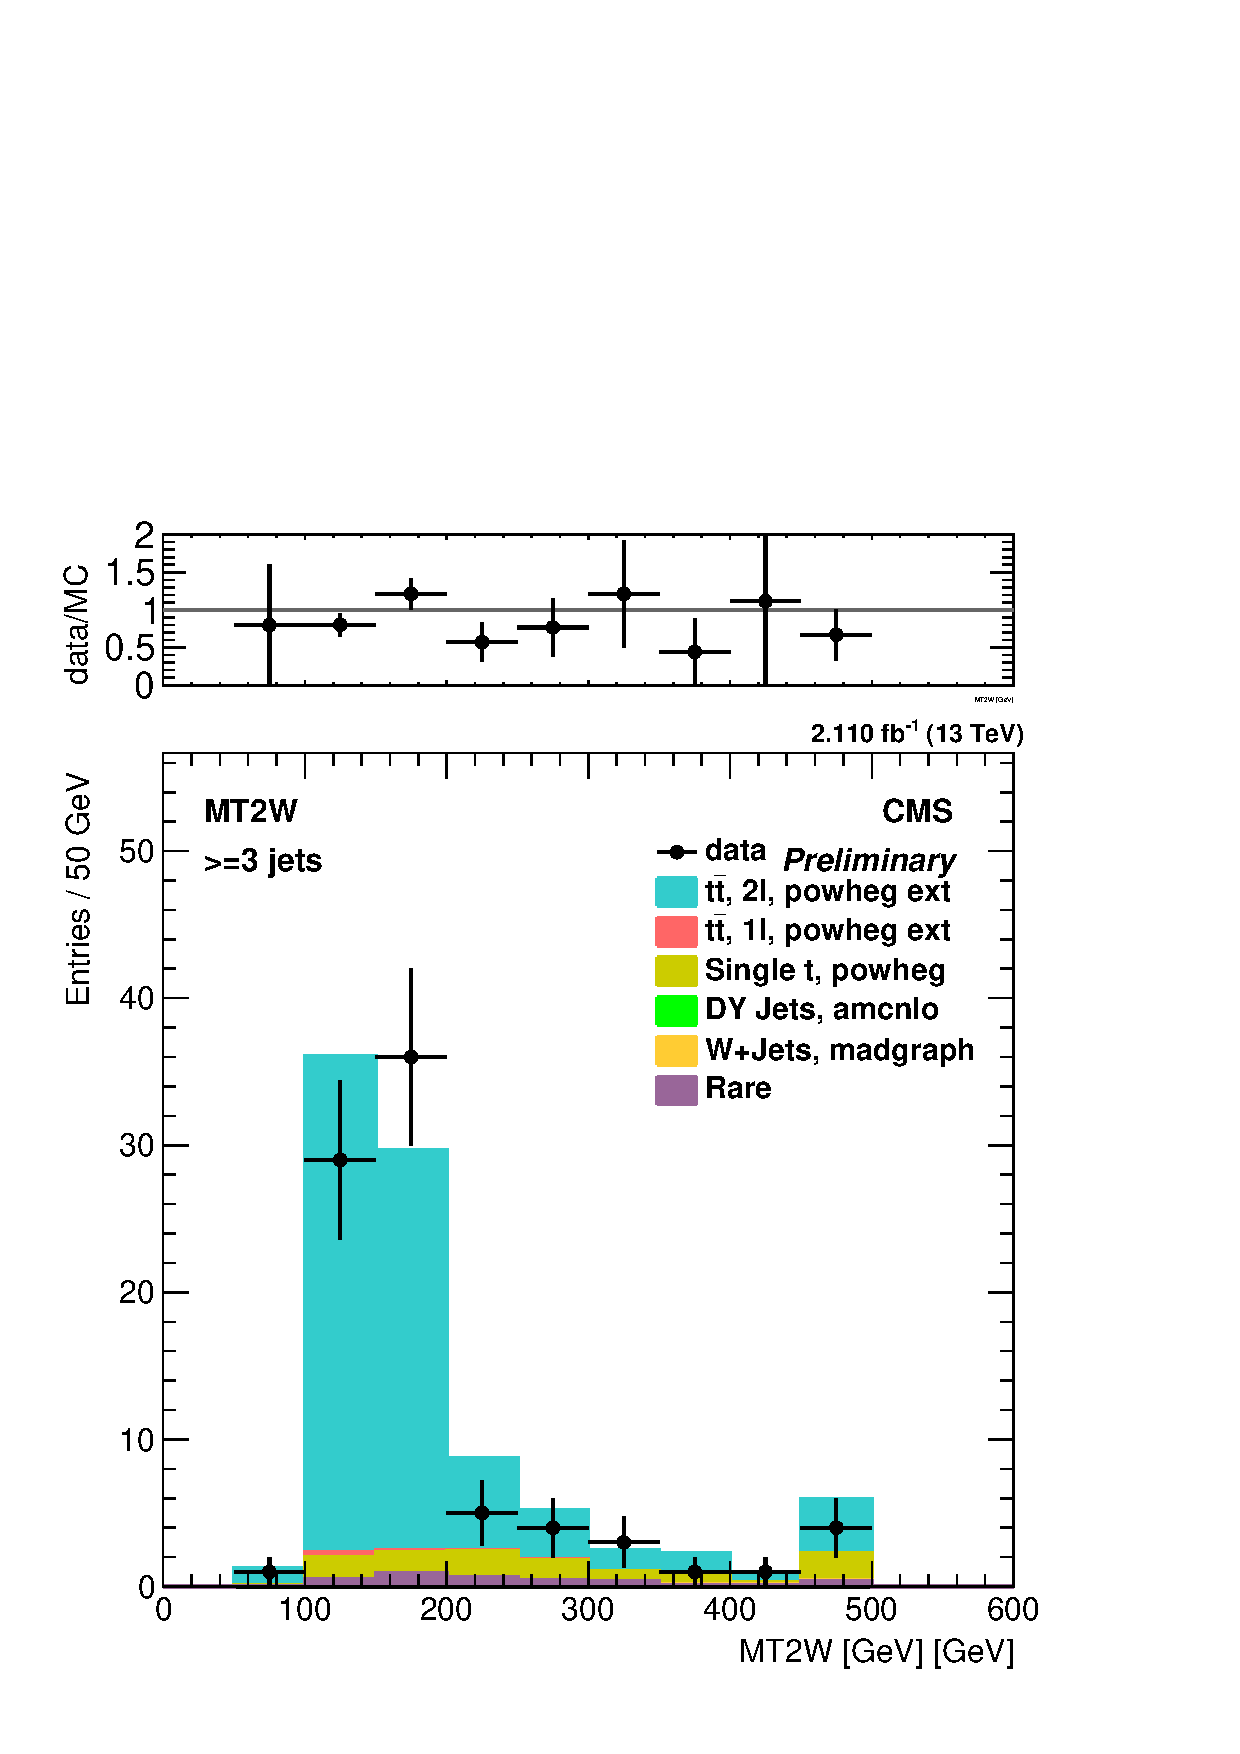
\includegraphics[width=0.45\textwidth]{plots_stop/data_MC_plot__byProductionMode__mt2w__ge3j_ge250met__linScale.pdf}
\caption{\label{fig:dilepton} Good agreement is observed in the dilepton control region for the \MET and \MTtW distributions.}
\end{figure}

$\ttbar\rightarrow 2l$ only contributes to the signal regions with 3 or 4 jets if additional jets from initial-or final-state-radiation are present.  Sometimes also a hadronic tau can be misidentified as an additional jet.  The modeling of the jet multiplicity is checked in a high-purity dedicated $e-\mu$ control region with at least two (b-tagged) jets.  The scale-factors extracted from the comparison between data and simulation are 1.10+/- 0.06 in case we ask for exactly 3 jets and 0.94+/0.06 when we ask for at least 4 jets.  These scale-factors are also checked to be constant with increasing \MET requirements within the statistical uncertainty.

We rely on the simulation for the \MET modeling.  Therefore it is important that we check that the \MET resolution is well described in simulation.  Changing the resolution can lead to a different \MET spectrum and thus bin-to-bin migrations between the search bins. The uncertainty due to the \MET resolution is estimated by comparing the $\gamma$+jets sample in data and simulation.  The photon \pt spectrum is reweighted to match that from the neutrinos in the background simulation sample.  In case of $\ttbar\rightarrow 2l$ this will be the $\nu\nu$ $\pt$ spectrum.    We then add the transverse momentum of the photon to the MET and then compare the resulting spectrum.   The differences between data and simulation are then applied to the $\ttbar\rightarrow 2l$ simulation and are used to assess the systematic uncertainties. Validating the \MET resolution is also important for the one lepton backgrounds, where we rely on the simulation to determine the transfer factors used for the W+Jets prediction and to assess the small $\ttbar\rightarrow 1l$ contribution.  The systematic uncertainties of the method are described in Sec.~\ref{sec:syst}.  The final systematic uncertainty varies between 20 and 47\% for the dilepton backgrounds.

\subsection{One lepton background}\label{sec:onelepton}
After applying the transverse mass cut, the main SM background with one real lepton comes from direct W production.  This background is estimated by using a control region with no b-tagged jets in the event.  The other cuts for this region are identical to the baseline selection. For low \MTtW the SM background is completely dominated by the lost lepton background and the one lepton background accounts for less than 10\% of the background everywhere.  A data-driven method is not required and the simulation is used to predict the background.   

For high \MTtW we estimate the W+Jets background separately in two bins of exactly 3 jets and at least 4 jets.  The full \MT distribution for the 0b-tag control region is shown on Fig~\ref{fig:MT}. There is reasonable agreement between data and simulation across the \MT spectrum.   For the large \MT ($>150 \GeV$) region, roughly 35\% of the control regions consists of dileptonic ttbar and invisible Z backgrounds.  Those backgrounds are subtracted to perform the W+Jets estimation, with a 50\% uncertainty assigned to this subtraction.   We then extrapolate the W+Jets yield from the sideband to the signal regions by a transfer factor from simulation to perform the b-tag and \MET extrapolation.  B-tagging scale factors are applied and also the \MET resolution effects are studied with the study described in Sec.~\ref{sec:dilepton}.  After assessing all sources of systematic uncertainties as described in Sec.\ref{sec:syst} , the total uncertainty on the W+Jet estimate varies  between 50 and 70\%.

\begin{figure}[h]
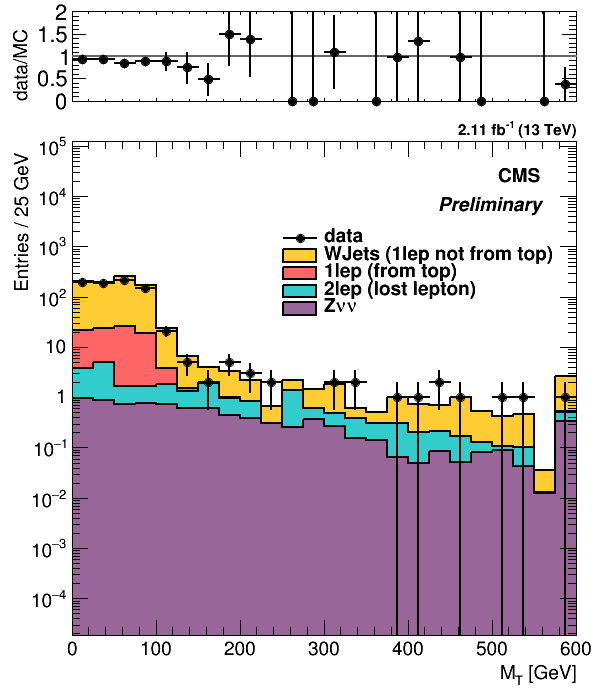
\includegraphics[width=0.44\textwidth]{plots_stop/MTDist_3jets.png}
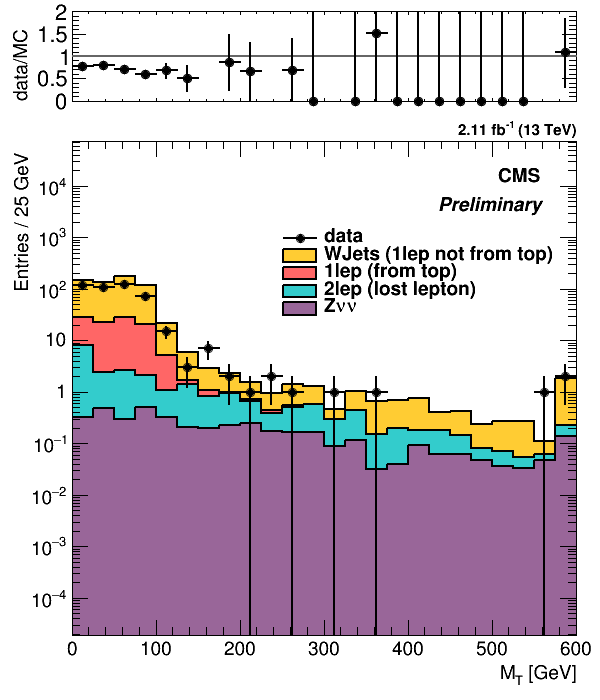
\includegraphics[width=0.44\textwidth]{plots_stop/MTDist_4jets.png}
\caption{\label{fig:MT} Distribution of \MT distribution for 3 jets (left) and $\ge$ 4 jets (right) in the b-vetoed control region with \MET $>$ 250\GeV. Good agreement between data and simulation is seen for the full distribution.}
\end{figure}

The $\ttbar\rightarrow 1l$ background is always negligible compared to the other backgrounds.  Therefore we rely on simulation to estimate the background.  The main uncertainty on this estimate is the \MET resolution since the resolution effects could enhance the \MT tail.  The \MET resolution study shows that the resolution could be mismodeled by as much as 10\%.  We vary the resolution conservatively by 20\% and take the largest discrepancy in a single \MET bin (100\%) as the systematic uncertainty on the \ttbar estimate.  
\subsection{Rare Standard Model backgrounds}
The analysis also suffers from rare SM backgrounds, like $\ttbar$W, \ttbar$Z and VV.  It turns out that around 80\% of this background is due to \ttbar$Z with the Z decaying to two neutrino's ($Z\rightarrow\nu\nu$) and this ratio increases with an increasing \MET cut.  Possible control regions, e.g. trileptons, have too few events in the current dataset so these backgrounds are estimated using simulation.  We assess all the theoretical and experimental uncertainties (Sec.~\ref{sec:syst}) and end up with a systematic uncertainty of 15-26\% depending on the exact search region.
